\subsection{Cahier des charges}

Dans le but de développer la bibliothèque, nous avons établi un cahier des charges présentant et définissant les trois ensembles de fonctionnalités qui la constitue :
\begin{itemize}
\item Pré-traitement des images
\item Détection des évolutions d'un dessin
\item Reconnaissance des formes dessinées
\end{itemize}

\subsubsection{Pré-traitement}

Tout traitement sur une image nécessite d'effectuer un certain nombre de pré-traitements afin d'améliorer la qualité de cette image. Cette étape a pour but de favoriser l'obtention de bons résultats lors de la phase de traitement.\\

La bibliothèque devra permettre d'appliquer aisément un certain nombre de filtres, notamment :

\begin{description}
\item[Filtre morphologique] Optimisation des méthodes de template matching;
\item[Binarisation] Permettre de trouver les différences qui existent entre deux images;
\item[Correction de couleur] Balance des blancs, permet d'annuler la coloration globale de l'image, dépendante de l'éclairage de la scène (lumière du jour, lumière artificielle, etc ...);
\item[Filtrage par couleur] Récupérer uniquement les formes dessinées avec une couleur précise.
\end{description}

La bibliothèque devra permettre de développer de nouveaux filtres. Tous les filtres devront pouvoir être utilisés de la même manière afin d'en simplifier l'usage, ils devront avoir une interface commune.

\clearpage
\subsubsection{Détection des évolutions d'un dessin}

La première fonctionnalité de la bibliothèque est de permettre la récupération de plus haute qualité possible d’un dessin à différents moments. Les moments de prise de vue du dessin seront considérés comme idéaux, pas de mains, ni d'objets dans le champ de prise de vue.

On cherche ici à permettre le développement d'applications permettant d'observer les moments clés de la création d'un dessin sans perturber le travail de l'artiste, c'est à dire, éviter de scanner la feuille.

\paragraph{Performance\protect\footnotemark[1]\\}
La bibliothèque devra permettre l'analyse d'image à une cadence de 2 à 3 images par seconde. Le but ici n'est pas la performance mais bien la qualité de l'analyse.
Les images à traiter seront acquises en haute définition, un minimum de 1080 lignes de 1920 pixels, ce qui correspond à la résolution d'un flux vidéo HDTV 1080p.


\subsubsection{Reconnaissance des formes dessinées}
La deuxième fonctionnalité de la bibliothèque est de reconnaître, dans un flux vidéo, des dessins ou pictogrammes pré-enregistrés. 

Différentes méthodes pourront être développées selon que les formes à reconnaître dans l'image sont simples (e.g. : un carré, un cercle) ou complexe (e.g. : un visage).

On utilisera par exemple :

\begin{itemize}
\item Template Matching : Mise en correspondance d'une image avec une image de référence pour la détection de formes simples.
\item Feature detection : Utilisation de caractéristiques invariantes dans l'image pour la reconnaissance de formes complexes (e.g. : descripteurs SURF).
\end{itemize}

\paragraph{Performance\protect\footnotemark[1]\\}
La bibliothèque devra permettre l'analyse d'image à une cadence de 30 à 60 images par seconde. Le but ici est d'effectuer de l'analyse sur un flux vidéo temps réel, de basse qualité.
Les images à traiter seront acquises en basse qualité, on prendra comme base des vidéos de résolution 480 lignes de 640 pixels, ce qui correspond au format VGA.

\footnotetext[1]{Les problématiques de performance sont secondaires, l'objectif principal est de développer une bibliothèque qui fonctionne.}

\clearpage
\subsection{Planning}
Le projet s'est déroulé suivant un planning se découpant en deux phases principales : une phase de préparation et d'organisation du projet et une phase de développement, de tests et de fin de projet.\\

La phase de préparation et d'organisation, présentée dans le diagramme de Gantt ci-après, est divisée en deux tâches :
 \begin{itemize}
 \item \'Etablissement du cahier des charges par l'ensemble du groupe
 \item \'Etude de l'existant. Cette dernière étant subdivisée en deux sous-tâches : 
	 \begin{itemize}
		\item \'Etude des methodes de prétraitements d'image, réalisé par Fabien Ridel et Jun Wen;
		\item \'Etude des méthodes d'extraction de nouveautés et de de reconnaissance de forme dans l'image, réalisé par Tomy Manson et Nicolas Mestreau.
	\end{itemize}
\end{itemize} 

\begin{center}
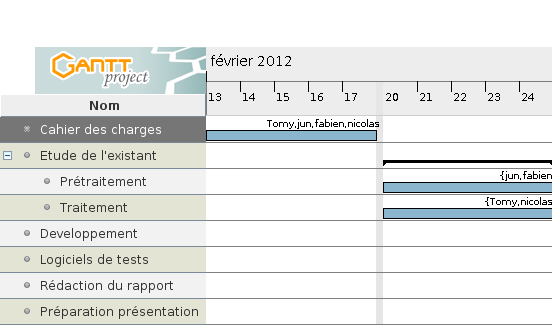
\includegraphics[width=\textwidth]{gantt1.png}
\captionof{figure}{Planning taches préparatoire}
\end{center}

\clearpage
La phase suivante, présentée dans le diagramme de Gantt ci-après, est la phase de développement de la bibliothèque, de programme de démonstration et de tests. Nous incluons dans cette phase la rédaction du rapport et la préparation de la présentation, qui constituent la fin de projet.

\begin{center}
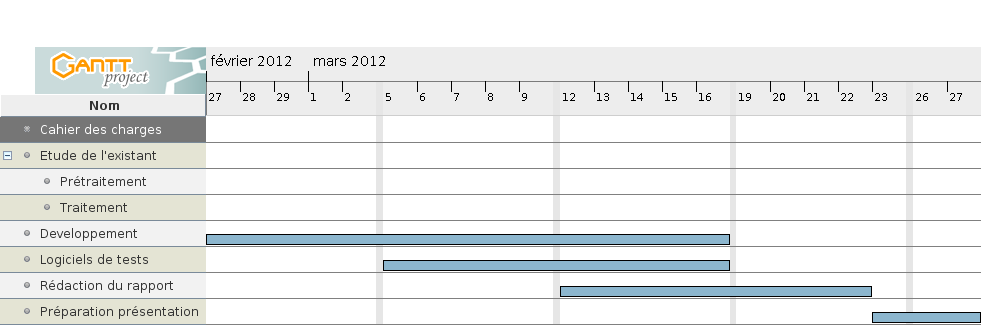
\includegraphics[width=\textwidth]{gantt2.png}
\captionof{figure}{Planning de dévelopement et de fin de projet}
\end{center}